\documentclass[11pt]{article}
\usepackage{amssymb,amsmath,times}
\usepackage[T1]{fontenc}
\usepackage{mathptmx}
\usepackage[dvipsnames]{xcolor}
\usepackage{graphicx}
\usepackage{fancyhdr}
\usepackage{multirow}
%\usepackage{cite}
\usepackage[numbers,sort&compress]{natbib}
\usepackage{color}
%\usepackage{natbib}
\usepackage[nolist]{acronym}
% Soumen's packages
\usepackage[plainpages=false,pdfpagelabels,colorlinks=true]{hyperref}
%\usepackage{hyperref}
\usepackage[latin1]{inputenc}
\usepackage{grffile}
\usepackage{multirow}
\usepackage{adjustbox}
%subfiles
\usepackage{subfiles}
\usepackage[small,compact]{titlesec}
\usepackage[font=small]{caption}
\usepackage{multirow}
\usepackage{afterpage}
\usepackage{multicol}
%\usepackage{draftwatermark}
\usepackage[normalem]{ulem}
\usepackage{wrapfig}
\usepackage{pdfpages}

%crossing reference footnote
\usepackage{cleveref}
\crefformat{footnote}{#2\footnotemark[#1]#3}

%% [TJP] Display the labels (turn off for final version)
%\usepackage[right]{showlabels}
%\renewcommand{\showlabelfont}{\scriptsize\color{blue}}

%% [TJP] Number figures and tables by section
\usepackage{chngcntr}
\counterwithin{figure}{section}
\counterwithin{table}{section}

%% [TJP] Compact itemize lists
\usepackage{enumitem}
\setitemize{noitemsep,topsep=0pt,parsep=0pt,partopsep=0pt}
\setenumerate{noitemsep,topsep=0pt,parsep=0pt,partopsep=0pt}

%% [TJP] Format for citation numbers
\renewcommand{\citenumfont}[1]{\textit{#1}}

%% [TJP] Customize table and figure captions
\usepackage[font={small},margin=0em]{caption}

%% [TJP] Customize section and subsection title format
\usepackage[small,compact]{titlesec}
\titleformat{\section}
  {\normalfont\sffamily\Large\bfseries\color{MidnightBlue}\filcenter}
  {\thesection}{1em}{}
\titleformat{\subsection}
  {\normalfont\sffamily\large\bfseries\color{MidnightBlue}}
  {\thesubsection}{1em}{}
\titleformat{\subsubsection}
  {\normalfont\sffamily\bfseries\itshape\color{MidnightBlue}}
  {\thesubsubsection}{0.5em}{}
\titleformat{\paragraph}[runin]
  {\normalfont\sffamily\bfseries\color{MidnightBlue}}
  {\theparagraph}{}{$\bullet$\hskip 0.5em}
\titlespacing*{\subsection}{0pt}{6pt}{2pt}
\titlespacing*{\subsubsection}{0pt}{4pt}{2pt}

%% [TJP] Commands to add disclaimer at the bottom of pages with dollar signs on them
\fancypagestyle{cost}{\fancyhf{}\renewcommand{\headrulewidth}{0pt}\fancyfoot[C]{\thepage\\\textit{\sf\color{gray}The cost information contained in this document is of a budgetary and planning nature and is intended for informational purposes only.}}}
\newcommand\costfootnote{\pagestyle{cost}}

% add watermark
%\usepackage[nostamp]{draftwatermark} % remove watermark
%\SetWatermarkText{DRAFT}
%\SetWatermarkScale{1}
%\SetWatermarkLightness{.87}

% Letter-size paper

\newlength{\pagewidthA}
\newlength{\pageheightA}
\setlength{\pagewidthA}{8.5in}
\setlength{\pageheightA}{11in}

% Double-page paper

\newlength{\pagewidthB}
\newlength{\pageheightB}
\setlength{\pagewidthB}{17in}
\setlength{\pageheightB}{11in}

\newlength{\stockwidth}
\newlength{\stockheight}

\usepackage{geometry}
\newcommand{\generatePageLayouts}{%
  \newgeometry{layoutwidth=\pagewidthA,layoutheight=\pageheightA, left=1in,right=1in,top=1in,bottom=1in}
  \savegeometry{LayoutPageA}

  \newgeometry{layoutwidth=\pagewidthB,layoutheight=\pageheightB, left=1in,right=1in,top=.75in,bottom=1in}
  \savegeometry{LayoutPageB}
}


\newcommand{\switchToLayoutPageA}{%
  % switch page size first:
  \pdfpagewidth=\pagewidthA \pdfpageheight=\pageheightA % for PDF output
  \paperwidth=\pagewidthA \paperheight=\pageheightA     % for TikZ
  \stockwidth=\pagewidthA \stockheight=\pageheightA % hyperref (memoir)?!
  \loadgeometry{LayoutPageA} % note; \loadgeometry may reset paperwidth/h!
}

\newcommand{\switchToLayoutPageB}{%
  % switch page size first:
  \pdfpagewidth=\pagewidthB \pdfpageheight=\pageheightB % for PDF output
  \paperwidth=\pagewidthB \paperheight=\pageheightB     % for TikZ
  \stockwidth=\pagewidthB \stockheight=\pageheightB % hyperref (memoir)?!
  \loadgeometry{LayoutPageB} % note; \loadgeometry may reset paperwidth/h!
}

% define formatting
%\pagestyle{empty}
\parindent=0pt
\topmargin=0.in \headheight=0in \headsep=-0.1in \textheight=9.2in
\textwidth=6.5in \oddsidemargin=0in

% command to compress figure captions slightly.
\newcommand{\captiontext}{\small \setlength{\baselineskip}{0.90\baselineskip}}



% define spacings
\def\p{\smallskip}
\def\sp{\vspace{0.15in}}
\def\spa{\vspace{0.3in}}
\def\spaa{\vspace{0.5in}}
\def\spaaa{\vspace{0.7in}}

% define shorthands for latex commands
\def\bei{\begin{itemize}}
\def\eei{\end{itemize}}

% define commonly used symbols
\def\et{{\it et al.\ }}
\def\degr{$^{\circ}$}
\def\arcsec{$^{\prime\prime}$}
\def\pp{\pi}

% define various names
\def\usk{ }
\def\max{MAX}
\def\maxima{MAXIMA}
\def\boom{BOOMERanG}
\def\arch{Archeops}
\def\maxboom{\maxima/\boom}
\def\planck{{\it Planck}}
\def\combat{COMBAT}
\def\cmb{CMB}
\def\cmba{CMBA}
\def\tic{Ticra}
\def\codef{CODE5}
\def\forecast{FORECAST}
\def\maxipol{MAXIPOL}
\def\hwp{HWP}
\def\ahwp{AHWP}
\def\wmap{WMAP}
\def\igb{IGB}
\def\apex{APEX}
\def\ebex{EBEX}
\def\squid{SQUID}
\def\ld{LD}
\def\ldii{LD-II}
\def\blast{BLAST}
\def\pb{\sc polarbear}
\def\pbsa{{\sc polarbear}/SA}
\def\spttg{SPT3G}
\def\ebextw{EBEX2013}
\def\ebexsk{EBEX-IDS}
\def\litebird{LiteBIRD}
\def\bicep{BKA}
\def\biceptwo{BICEP2}
\def\dfmux{DFMux}
\def\xsixf{$\times$64}
\def\xones{$\times$16}
\newcommand{\core}{\textit{\negthinspace CORE\/}}

% for systematics section
\newcommand{\suffix}{pdf} % for pdflatex
\newcommand{\pico}{PICO}
\newcommand{\prang}{\ensuremath{\alpha}}% Polarisation Rotation Angle
\newcommand{\arcmin}{\ensuremath{'}}
\newcommand{\degree}{\ensuremath{^o}}
\newcommand{\fsky}{f_{\rm sky}}
\newcommand{\EFH}[1]{\textcolor{red}{$\dagger${[#1]}$\dagger$}}


%define physics and cosmological notations
\def\het{$^{3}$He}
\def\hef{$^{4}$He}
\def\lnt{lN$_{2}$}
\def\wn{cm$^{-1}$}
\def\omeg{$\Omega$}
\def\omegb{$\Omega_{b}$}
\def\hubble{$H_{0}$}
\def\lamb{$\Lambda$}
\def\cl{$C_{\ell}$}
\def\micron{$\mu$m}
\def\microk{$\mu{\mbox{K}}$}
\def\microkrtsec{$\mu{\mbox{K}}\sqrt{\mbox{sec}}$}
\def\microkprthz{$\mu{\mbox{K}}/\sqrt{\mbox{Hz}}$}
\def\wattrthz{${\mbox{Watt}}\sqrt{\mbox{Hz}}$}
\def\voltprthz{${\mbox{Volt}}/\sqrt{\mbox{Hz}}$}
\def\sintheta{\mbox{$\sin\theta$}}
\def\bceti{$\beta$-ceti}
\def\etad{$\eta$-draconis}
\def\ruo2{RuO$_{2}$}
\def\tdot{$\dot{\theta}$}
\def\taub{$\tau_{b}$}
\def\degsq{deg$^2$}

% define polarization symbols parameters
\def\It{$I_{t}$}  
\def\sq{$Q$}
\def\su{$U$}
\def\dsu{$\Delta U$}
\def\dsq{$\Delta Q$}
\def\TT{$C_l^{\rm TT}$}
\def\TE{$C_l^{\rm TE}$}
\def\EE{$C_l^{\rm EE}$}
\def\BB{$C_l^{\rm BB}$}

% define math and vectors

\def\mathrelfun#1#2{\lower3.6pt\vbox{\baselineskip0pt\lineskip.9pt
  \ialign{$\mathsurround=0pt#1\hfil##\hfil$\crcr#2\crcr\sim\crcr}}}
\def\simlt{\mathrel{\mathpalette\mathrelfun <}}
\def\simgt{\mathrel{\mathpalette\mathrelfun >}}

\def\hatx{{\bf \hat n}}
\def\hatnprime{{\bf \hat n'}}
\def\hatnone{{\bf \hat n}_1}
\def\hatntwo{{\bf \hat n}_2}
\def\hatni{{\bf \hat n}_i}
\def\hatnj{{\bf \hat n}_j}
\def\vecx{{\bf x}}
\def\veck{{\bf k}}
\def\hatx{{\bf \hat x}}
\def\hatk{{\bf \hat k}}
\def\hatz{{\bf \hat z}}
\def\VEV#1{{\left\langle #1 \right\rangle}}
\def\cP{{\cal P}}
\def\noise{{\rm noise}}
\def\pix{{\rm pix}}
\def\map{{\rm map}}
\long\def\comment#1{}

% \newcommand{\beq}{\begin{equation}}
% \newcommand{\eeq}{\end{equation}}
% \newcommand{\bea}{\begin{eqnarray}}
% \newcommand{\eea}{\end{eqnarray}}
\newcommand\PRL{{\it Phys.~Rev.~Lett.}}
\newcommand\prl{{\it Phys.~Rev.~Lett.}}
\newcommand\ApJ{{\it Ap.~J.}}
\newcommand\apj{{\it Ap.~J.}}
\newcommand\ApJL{{\it Ap.~J.~Lett.}}
\newcommand\apjl{{\it Ap.~J.~Lett.}}
\newcommand\ApJS{{\it Ap.~J.~Suppl.}}
\newcommand\apjs{{\it Ap.~J.~Suppl.}}
\newcommand\PR{{\it Phys.~Rev.}}
\newcommand\PL{{\it Phys.~Lett.}}
\newcommand\MNRAS{{\it MNRAS}}
\newcommand\mnras{{\it MNRAS}}
\newcommand\MNRASL{{\it MNRAS\ Lett.}}
\newcommand\AnA{{\it Astron.~Astrophys.}}
\newcommand\BAAS{{\it Bull.~Am.~Astron.~Soc.}}
\newcommand\NP{{\it Nucl.~Phys.}}
\newcommand\RMP{{\it Rev.~Mod.~Phys.}}
\newcommand\ARAA{{\it ARAA}}
\newcommand\prd{{\it Phys.~Rev.~D.}}
\newcommand\plb{{\it Phys.~Lett.~B.}}
\newcommand\ao{{\it Appl.~Optics}}
\newcommand\aap{{\it Astron.~Astrophys.}}
\newcommand\aaps{{\it Astron.~Astrophys.~Suppl.}}
\newcommand\pasp{{\it Proc.~Ast.~Soc.~Pac.}}
\newcommand\josa{{\it J.~Opt.~Soc.~Am.}}
\newcommand\phr{{\it Phys. Reports}}
\newcommand\aj{{\it Astronomical Journal}}
\newcommand\jcap{{\it JCAP}}
\newcommand\apss{{\it ApSS}}

\newcommand{\comred}[1]{\textcolor{red}{#1}}
\newcommand{\comblue}[1]{\textcolor{blue}{#1}}

% Let's you define a command for both text and math mode. 
\newcommand{\wisk}[1]{{\ifmmode{#1}\else{$#1$}\fi}}



%-----------------------------------------------------------------------
% Tables
%-----------------------------------------------------------------------
\newbox\tablebox    \newdimen\tablewidth
\def\leaderfil{\leaders\hbox to 5pt{\hss.\hss}\hfil}
%
% use the following definition of \endPlancktable for ApJ style notes to tables, set to the 
%         width of the table
% \def\endPlancktable{\tablewidth=\wd\tablebox 
%
% use the following definitions of \endPlancktable and \endPlancktablewide for A&A style notes 
% set to one-column  or full-page width, respectively
\def\endPlancktable{\tablewidth=\columnwidth 
    $$\hss\copy\tablebox\hss$$
    \vskip-\lastskip\vskip -2pt}
\def\endPlancktablewide{\tablewidth=\textwidth 
    $$\hss\copy\tablebox\hss$$
    \vskip-\lastskip\vskip -2pt}
\def\tablenote#1 #2\par{\begingroup \parindent=0.8em
    \abovedisplayshortskip=0pt\belowdisplayshortskip=0pt
    \noindent
    $$\hss\vbox{\hsize\tablewidth \hangindent=\parindent \hangafter=1 \noindent
    \hbox to \parindent{$^#1$\hss}\strut#2\strut\par}\hss$$
    \endgroup}
\def\doubleline{\vskip 3pt\hrule \vskip 1.5pt \hrule \vskip 5pt}


%\setlength{\floatsep}{0.5\floatsep}
\setlength{\textfloatsep}{0.5\textfloatsep}
\setlength{\intextsep}{0.5\intextsep}
%\setlength{\floatsep}{0.5\floatsep}
%\setlength{\dblfloatsep}{0.5\dblfloatsep}
\setlength{\dbltextfloatsep}{0.5\dbltextfloatsep}
\setcounter{topnumber}{2}
\setcounter{bottomnumber}{2}
\setcounter{totalnumber}{4}
\renewcommand{\topfraction}{0.85}
\renewcommand{\bottomfraction}{0.85}
\renewcommand{\textfraction}{0.15}
\renewcommand{\floatpagefraction}{0.7}



\begin{document}

% generate page layouts first based on layoutwidth as page size;
  % don't switch actual page sizes yet:
  \generatePageLayouts{}

%\bibliographystyle{unsrtnat}

\setlength{\baselineskip}{0.96\baselineskip} %% measured, 5.0 lines/inch.  Can go to 0.96\baselineskip
\setlength{\parskip}{1.\parskip}
 \switchToLayoutPageA{}

%\tableofcontents

\pagenumbering{gobble}

%% Karl Young adding cover page as full page pdf.

%\includepdf{images/PICO_Cover_v2-4.pdf} %Full resolution cover
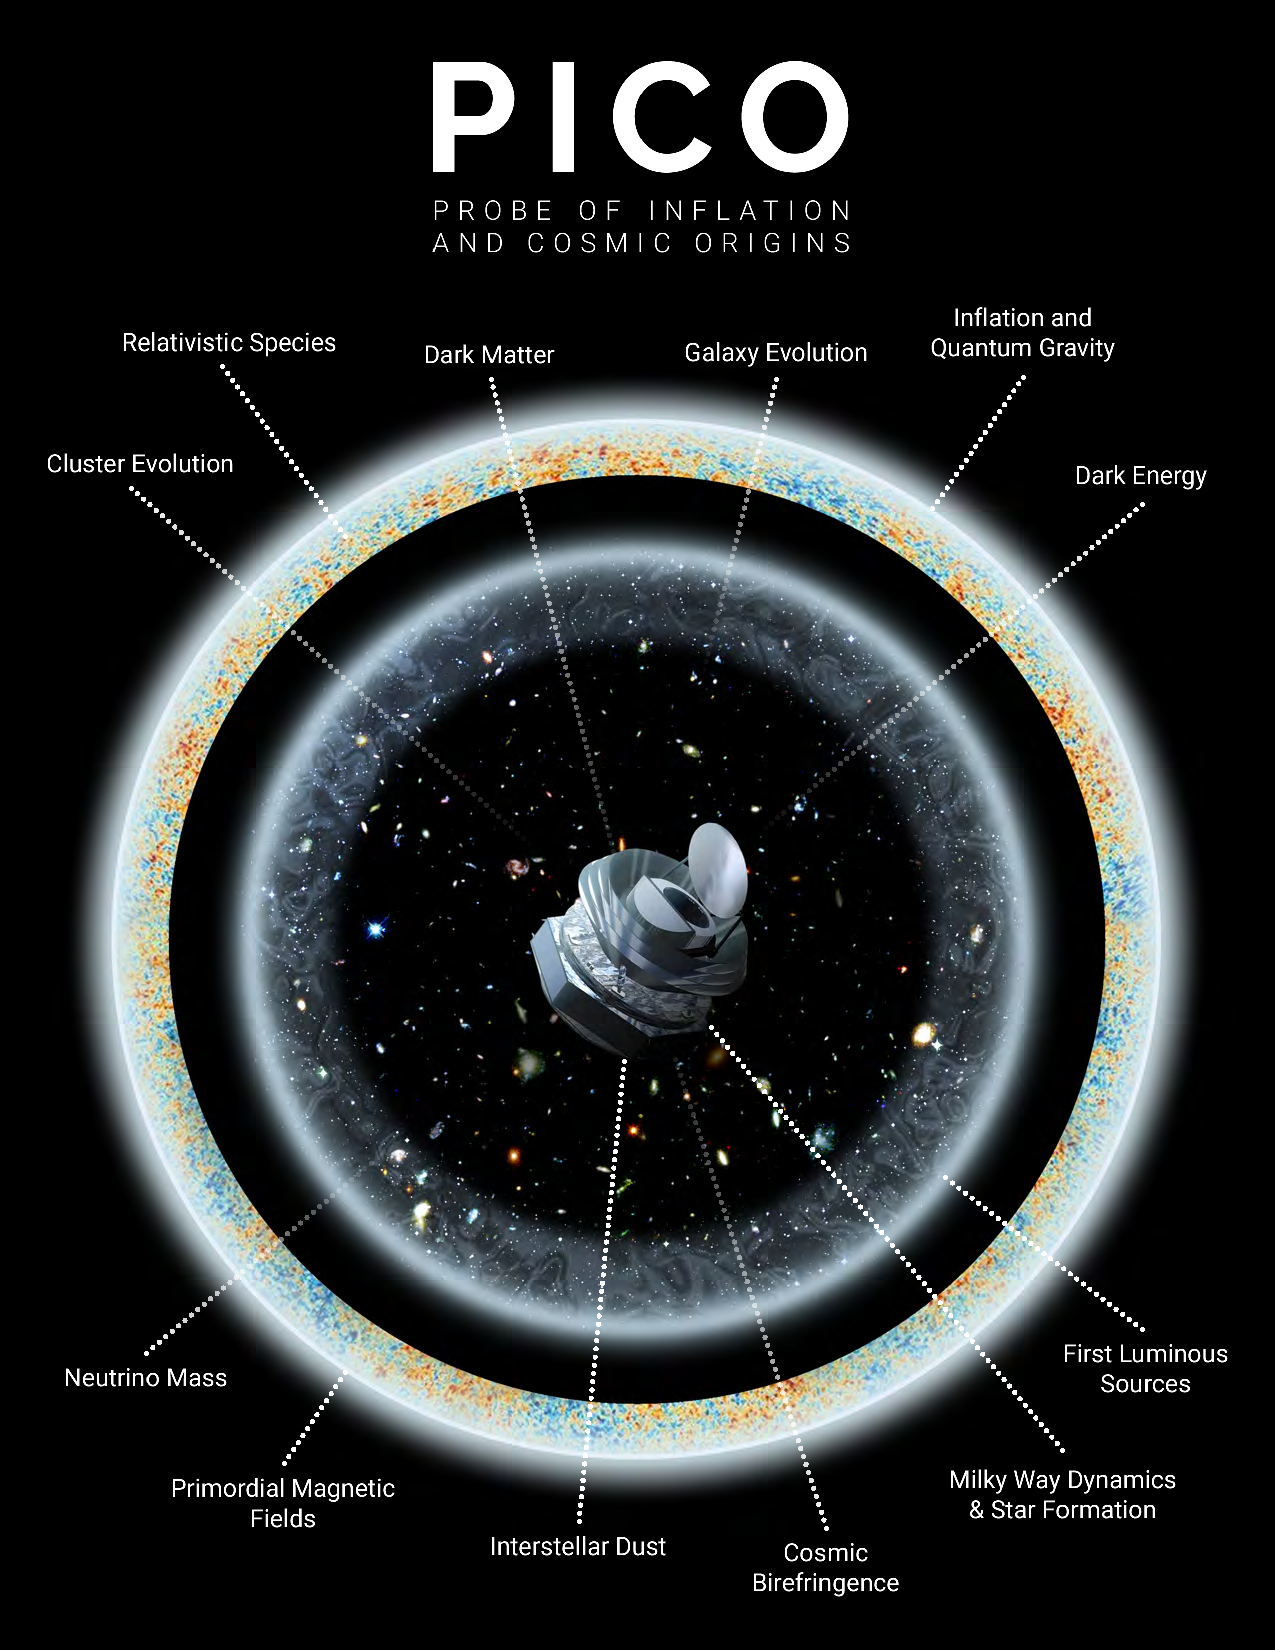
\includepdf{images/PICO_Cover_v6_s.pdf} %Low resolution cover for faster pdf. 


%%

%\LARGE{ \centerline{\bf{The Probe of Inflation and Cosmic Origins}}}
%\vspace{1.5in}
%%\Large{ \centerline{A Space Mission Study Report}}
%%\Large{ \centerline{December, 2018 }}
%%\vspace{0.5in}
%%\parindent = 0pt
%%\large{Principal Investigator:} \\
%%\large{Steering Committee:} \\
%%\large{Executive Committee:} \\
%%\large{Contributors:} \\
%%\large{Endorsers:} \\
%
%\normalsize
%
%\vspace{0.35in}
%\begin{figure}[!thb]
%%\begin{center}
%\hspace{-0.25in}
%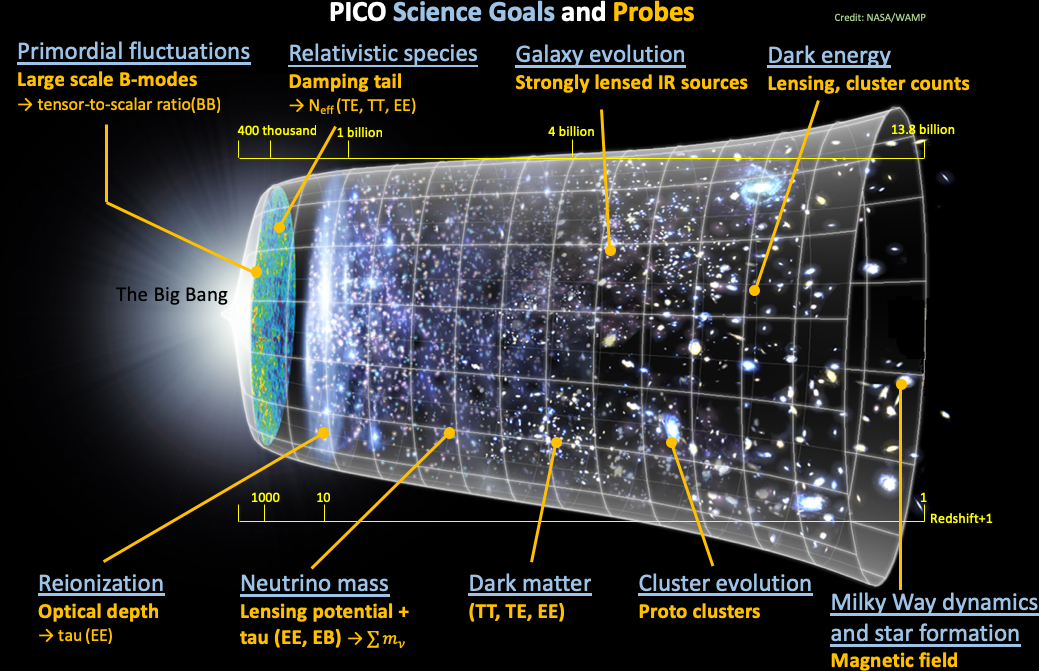
\includegraphics[width=7.0in]{images/PICO_science goals and probes.png}
%%\end{center}
%%\hspace{-0.15in}
%%\caption{PICO science goals and probes}
%\label{fig:PICOsci_probes}
%\end{figure}

\parindent = 15pt

\newpage
\newpage
%\twocolumn

%test figure in main file
%
\pagenumbering{roman} 
\setcounter{page}{1}

% Author list on seperate pages
\subfile{authorlist.tex}



\begin{centering}
{***}\\
\bigskip
{This research was funded by a NASA grant NNX17AK52G to the University of Minnesota / Twin Cities, by the Jet Propulsion Laboratory, California Institute of Technology, under a contract with the National Aeronautics and Space Administration, and by Lockheed Martin Corporation. \\ Substantial contributions to the development of PICO were volunteered by scientists at many institutions world-wide.  They are very gratefully acknowledged.} \\
\bigskip

{The information presented about the PICO mission concept is pre-decisional and is provided for planning and discussion purposes only.}\\
\bigskip

{The cost information contained in this document is of a budgetary and planning nature and is intended for informational purposes only.  It does not constitute a commitment on the part of JPL and/or Caltech.}\\
\bigskip

%{\copyright\ 2018. All rights reserved.}\\
\end{centering}
\newpage
{
             % KY: making table of contents links black instead of red.
\hypersetup{linkcolor=black}
\tableofcontents
}
\newpage
\pagenumbering{arabic} 
\setcounter{page}{1}
\setcounter{figure}{0}


\section{Executive Summary} % (2 pg, Hanany)}
\subfile{executive.tex}

\section{Science}
\label{sec:science}

\subsection{Introduction} % (1.5 pgs)}


%{\it NASA suggested table of contents says Science Intro or Landscape section should include: State of the Art in the Field ; Compelling Outstanding Questions; Needed Capabilities for Progress. }

\subfile{Introduction.tex}

%\vspace{-0.18in}

%\subsection{Science Objectives} % (17.5 pgs) }

%\vspace{-0.05in}




\subsection{Fundamental Physics} %(6 pgs)
\label{sec:fundamentalsci}
%\vspace{-0.05in}

\subfile{fundamentalsci.tex}

%\vspace{-0.05in}

% ------------

\subsection{Cosmic Structure Formation and Evolution} % (4 pgs)
\label{sec:extragalacticsci}
\subfile{extragalacticsci.tex}

% ------------

\subsection{Testing $\Lambda$CDM} % (3 pgs)
\label{sec:testinglcdm}
\subfile{testlcdm.tex}

% ------------


\subsection{Galactic Structure and Star Formation} % (3 pgs)
\label{sec:galacticsci}
\subfile{galacticsci.tex}

% ------------

\subsection{Legacy Surveys} % (2 pgs)
\label{sec:legacy}

%\begin{table}[]
\caption{\textbf{Cosmological Legacy Science}}\label{tab:STM2}
\footnotesize
\begin{tabular}{lll}
\noalign{\vskip 2mm}
\hline
\noalign{\vskip 2mm}    
% Header line 1
{\bf \hfil Catalog\hfil}&
{\bf \hfil Impact\hfil}&
{\bf \hfil Science\hfil}\\
% Line 1
\noalign{\vskip 2mm}    
\hline
\noalign{\vskip 1mm}    
\parbox[t]{1in}{1. Proto-Clusters}&
\parbox[t]{2.3in}{Discover >$100,000^a$ mm/sub-mm proto-clusters distributed over the sky and across redshift.  
\vspace{1mm}
\hrule
\vspace{1mm}
Current knowledge: \planck\ data expected to yield a few tens.}&
\parbox[t]{2.7in}{Probe the earliest observable dust-enshrouded galaxy clusters to determine the initial stages of their formation and evolution.}\\
% Line 2
\noalign{\vskip 1mm}    
\cline{2-3}
\noalign{\vskip 1mm}    
\parbox[t]{1in}{2. Strongly\\ Lensed Galaxies}&
\parbox[t]{2.3in}{Discover 4500$^a$ highly magnified dusty galaxies across redshift. 
\vspace{1mm}
\hrule
\vspace{1mm}
Current knowledge: 13 sources confirmed in \planck\ data; few hundred candidates in \textit{Herschel}, SPT and ACT data.$^c$}&
\parbox[t]{2.7in}{Learn about dark matter sub-structure in the lensing galaxies; probe star formation history in high-$z$ dust-enshrouded galaxies, a population in which star formation history cannot be probed in any other way.}\\
% Line 3
\noalign{\vskip 1mm}    
\cline{2-3}
\noalign{\vskip 1mm}    
\parbox[t]{1in}{3. High-$z$ Galaxy\\ Clusters}&
\parbox[t]{2.3in}{Find \comor{1000$^a$} mm/submm emitting clusters at $1 < z < 1.5$ and $\sim20$ at $z>2$. 
\vspace{1mm}
\hrule
\vspace{1mm}
Current knowledge: \planck\ and \textit{Herschel} identified mm/sub-mm emission of $\sim100$ known sources.}&
\parbox[t]{2.7in}{Probe star formation history at high $z$ and in dust-enshrouded environments.}\\
% Line 4
\noalign{\vskip 1mm}    
\cline{2-3}
\noalign{\vskip 1mm}    
\parbox[t]{1in}{4. Polarized Point\\ Sources}&
\parbox[t]{2.3in}{Detect \comor{4000$^{a,b}$} radio and dusty galaxies in polarization. 
\vspace{1mm}
\hrule
\vspace{1mm}
Current knowledge: \comor{Shaul checking w/ Gianfranco}}&
\parbox[t]{2.7in}{Determine the structure of magnetic fields in dusty galaxies, and the mechanism for relativistic jet formation in radio-loud galaxies; Determine the importance of polarized sources as a foreground for CMB polarization science.}\\
\noalign{\vskip 1mm}
\hline
\noalign{\vskip 1mm}
\end{tabular}
{\footnotesize
$^a$ Confusion (not noise) limited\\
$^b$ Noise and confusion limited\\
$^c$ Many \textit{Planck} candidates are not expected to be real because of confusion. \textit{Herschel}, SPT, and ACT source candidates are expected to be real. PICO source candidates will mostly be real.}
\end{table}
 

\subfile{Legacy.tex}


% ------------

\subsection{Signal Separation}%  (4 pages)}
\label{sec:signal_separation}

\subfile{foregrounds.tex}

% ------------

\subsection{Systematic Uncertainties}%  (3 pgs)}
\label{sec:systematics}
\subfile{systematics.tex}

% ------------

\subsection{Complementarity with Sub-Orbital Measurements}
\label{sec:complementarity}

\subfile{complementarity.tex}

% ------------

\subsection{Measurement Requirements} % (2 pgs)}
\label{sec:requirements}

\subfile{requirements.tex}

%\newpage

% ------------

%\section{Instrument (6 pgs, Hanany \& Transgrud)}

%\subfile{instrument.tex}

% ------------

%\section{Mission (5 pgs, Trangsrud)}

%\subfile{mission.tex}

% ------------

%\section{Technology Maturation (4 pgs, O'Brient \& Trangsrud)}

%\subfile{technology.tex}

% ------------

%\section{Management, Risk, Heritage, and Cost (4 pgs, Trangsrud)}

%\subfile{cost.tex}

% ------------
 \subfile{pico-eng-converted.tex}

\newpage
\def\bibfont{\footnotesize}
\setlength{\bibsep}{1pt}
\bibliographystyle{IEEEtranN}
\bibliography{mybib,pico-report}


\begin{acronym}
    %A
    \acro{ACS}{attitude control system}
    \acro{ADC}{analog-to-digital converters}
    \acro{ADS}{attitude determination software}
    \acro{AHWP}{achromatic half-wave plate}
    \acro{AMC}{Advanced Motion Controls}
    \acro{ARC}{anti-reflection coatings}
    \acro{ATA}{advanced technology attachment}
    %B
    \acro{BAO}{barion acoustic oscillations}
    \acro{BRC}{bolometer readout crates}
    \acro{BLAST}{Balloon-borne Large-Aperture Submillimeter Telescope}
    %C
    \acro{CANbus}{controller area network bus}
    \acro{CIB}{cosmic infrared background}
    \acro{CMB}{cosmic microwave background}
    \acro{CMM}{coordinate measurement machine}
    \acro{CSBF}{Columbia Scientific Balloon Facility}
    \acro{CCD}{charge coupled device}
    %D
    \acro{DAC}{digital-to-analog converters}
    \acro{DASI}{Degree~Angular~Scale~Interferometer}
    \acro{dGPS}{differential global positioning system}
    \acro{DfMUX}{digital~frequency~domain~multiplexer}
    \acro{DLFOV}{diffraction limited field of view}
    \acro{DSP}{digital signal processing}
    %E
    \acro{EBEX}{E~and~B~Experiment}
    \acro{EBEX2013}{EBEX2013}
    \acro{ELIS}{EBEX low inductance striplines}
    \acro{ETC}{EBEX test cryostat}
    %F
    \acro{FDM}{frequency domain multiplexing}
    \acro{FPGA}{field programmable gate array}
    \acro{FCP}{flight control program}
    \acro{FOV}{field of view}
    \acro{FWHM}{full width half maximum}
    %G
    \acro{GPS}{global positioning system}
    %H
    \acro{HDPE}{high density polyethylene}
    \acro{HIM}{high index materials}
    \acro{HWP}{half-wave plate} 
    %I
    \acro{IA}{integrated attitude}
    \acro{IGW}{inflationary gravity wave} 
    \acro{ILC}{independent linear combination}
    \acro{IP}{instrumental polarization} 
    %J
    \acro{JSON}{JavaScript Object Notation}
    %L
    \acro{LDB}{long duration balloon}
    \acro{LED}{light emitting diode}
    \acro{LCS}{liquid cooling system}
    \acro{LC}{inductor and capacitor}
    \acro{LZH}{Lazer Zentrum Hannover}
%M
    \acro{MCP}{multi-color pixel}
    \acro{MSM}{millimeter and sub-millimeter}    
    \acro{MLR}{multilayer reflective}
    \acro{MAXIMA}{Millimeter~Anisotropy~eXperiment~IMaging~Array}
    %N
    \acro{NASA}{National Aeronautics and Space Administration}
    \acro{NDF}{neutral density filter}
    %P
    \acro{PCB}{printed circuit board}
    \acro{PE}{polyethylene}
%    \acro{PTFE}{polytetrafluoroethylene}
    \acro{PME}{polarization modulation efficiency}
    \acro{PSF}{point spread function}
    \acro{PV}{pressure vessel}
    \acro{PWM}{pulse width modulation}
    %R
    \acro{RMS}{root mean square}
%S
    \acro{SLR}{single layer reflective}
    \acro{SMB}{superconducting magnetic bearing}
    \acro{SNR}{Signal to noise ratio}
    \acro{SQUID}{superconducting quantum interference device}
    \acro{SQL}{structured query language}
    \acro{STARS}{star tracking attitude reconstruction software}
    \acro{SWS}{sub-wavelength structures}
%T
    \acro{TES}{transition edge sensor}
    \acro{TDRSS}{tracking and data relay satellites}
   \acro{TM}{transformation matrix}
% U
    \acro{UHMWPE}{ultra high molecular weight polyethylene}   
    \acro{UMN}{University of Minnesota}
    
\end{acronym}


\end{document}

%\begin{figure}[!htb]
%\centering
%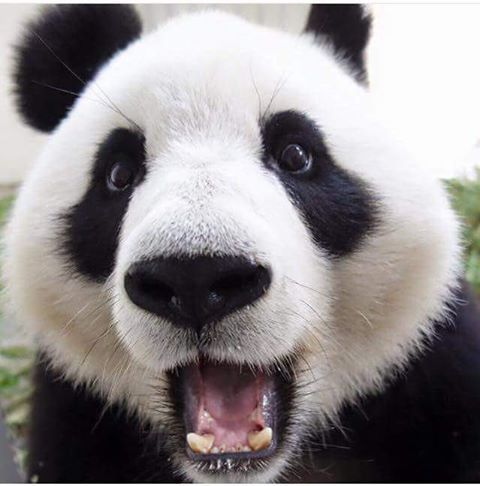
\includegraphics[width=4cm]{images/example0}
%\caption{example0}
%\label{fig:im_1}
%\end{figure}

